\subsection{Задачи с III семинара}
\subsubsection*{\xmark Задача 4.10}


% \begin{wrapfigure}{r}{0.4\textwidth}
%   \begin{center}
%         \vspace{-20 mm}
%         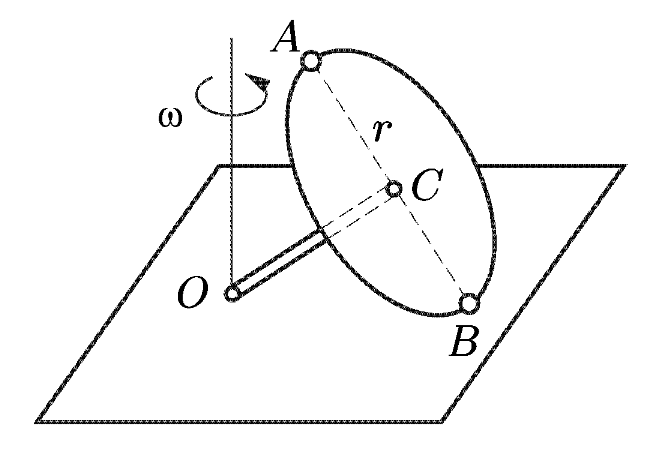
\includegraphics[width=0.9\linewidth]{img/4_10.png}
%   \end{center}
%     \caption{К задаче 4.10}
% \end{wrapfigure}

Диск катится без проскальзывания. 
$$
    \underbrace{\vc{v}_B}_{=0} = \underbrace{\vc{v}_O}_{=0} + \vc{\Omega} \times \vv{OB}
    \hspace{0.5cm}\Rightarrow \hspace{0.5cm}\vc{\Omega} || \vv{OB}.
$$
Также
\begin{align*}
    \vc{v}_C &= \vc{\Omega} \times \vv{BC} \\
    \vc{v}_C &= \vc{\Omega} \times \vv{OC} = \vc{\omega} \times \vv{OC}.  
\end{align*}

% ДОДЕЛАТЬ!!!
